%% IndustriConnect: A Model Context Protocol Suite for AI-Assisted Industrial Automation
%% arXiv submission — eess.SY (cross-list: cs.SE, cs.AI)
%%
%% AUTHOR NOTE: Replace all [Author N], [Affiliation N], [email N] placeholders before submission.
%% FIGURE NOTE:  Generate figures using the prompts in figures/prompts/, place PNGs in figures/.
%% REFERENCE NOTE: Verify all references against the actual publications before submission.

\documentclass[11pt,a4paper]{article}

%% ─── Packages ────────────────────────────────────────────────────────────────
\usepackage[margin=1in]{geometry}
\usepackage{microtype}
\usepackage{amsmath,amssymb}
\usepackage{graphicx}
\usepackage[numbers,sort&compress]{natbib}
\usepackage[colorlinks=true,linkcolor=blue,citecolor=blue,urlcolor=blue]{hyperref}
\usepackage{booktabs}
\usepackage{xcolor}
\usepackage{url}
\usepackage{authblk}
\usepackage{enumitem}
\usepackage{caption}
\usepackage{subcaption}

%% ─── Code listings ───────────────────────────────────────────────────────────
\usepackage{listings}
\definecolor{codebg}{rgb}{0.96,0.96,0.96}
\definecolor{codeframe}{rgb}{0.75,0.75,0.75}
\definecolor{commentcolor}{rgb}{0.4,0.4,0.4}
\definecolor{keywordcolor}{rgb}{0.0,0.3,0.6}
\definecolor{stringcolor}{rgb}{0.1,0.5,0.1}

\lstdefinestyle{jsonStyle}{
  language=,
  basicstyle=\ttfamily\small,
  backgroundcolor=\color{codebg},
  frame=single,
  rulecolor=\color{codeframe},
  breaklines=true,
  captionpos=b,
  numbers=none,
  showstringspaces=false,
}

\lstdefinestyle{pythonStyle}{
  language=Python,
  basicstyle=\ttfamily\small,
  backgroundcolor=\color{codebg},
  frame=single,
  rulecolor=\color{codeframe},
  keywordstyle=\color{keywordcolor}\bfseries,
  stringstyle=\color{stringcolor},
  commentstyle=\color{commentcolor}\itshape,
  breaklines=true,
  captionpos=b,
  numbers=left,
  numberstyle=\tiny\color{gray},
  showstringspaces=false,
}

%% ─── Figure placeholder helper ───────────────────────────────────────────────
%% When figures are not yet generated, this renders a labelled placeholder box.
%% Replace with \includegraphics once images are placed in figures/.
\newcommand{\figplaceholder}[2]{%
  \begin{center}
    \fbox{\parbox{0.88\linewidth}{%
      \centering\vspace{1.4cm}
      \textbf{\small Figure: #1}\\[0.4em]
      \textit{\small #2}
      \vspace{1.4cm}%
    }}%
  \end{center}%
}

%% ─── Title and authors ───────────────────────────────────────────────────────
\title{\textbf{IndustriConnect: A Model Context Protocol Suite\\
       for AI-Assisted Industrial Automation}}

\author[1]{[Author 1 Name]}
\author[2]{[Author 2 Name]}
% Add additional \author[N]{...} entries as needed
\affil[1]{[Department], [University / Institution 1], [City, Country]\\
         \texttt{[author1@example.com]}}
\affil[2]{[Department], [University / Institution 2], [City, Country]\\
         \texttt{[author2@example.com]}}

\date{\today}

%% ─── Document ────────────────────────────────────────────────────────────────
\begin{document}

\maketitle

%% ─── Abstract ────────────────────────────────────────────────────────────────
\begin{abstract}
AI assistants built on large language models (LLMs) excel at reasoning and
workflow orchestration but cannot natively communicate with operational
technology (OT) devices. We present \textbf{IndustriConnect}, an open-source
suite of Model Context Protocol (MCP) servers that exposes ten major industrial
protocols—Modbus, OPC~UA, MQTT/Sparkplug~B, BACnet, DNP3, EtherCAT,
EtherNet/IP, PROFIBUS, PROFINET, and Siemens~S7comm—as structured AI tools.
Each module follows a three-layer architecture: an MCP client issues tool calls,
a Python server translates them into native protocol operations, and real or
simulated field devices execute them. The suite provides a unified response
envelope for cross-protocol consistency, built-in device simulators for
hardware-free development, and a companion web console for multi-server
management. Together, these components let AI agents read process values, write
setpoints, and orchestrate diagnostics across heterogeneous industrial
environments without custom integration middleware.
\end{abstract}

\textbf{Keywords:} Industry MCP; Industry IOT; Industry AI Agents; Industry Protocols.

\vspace{1em}
\noindent\textit{arXiv categories:} eess.SY (primary); cs.SE; cs.AI

\newpage

%% ─── 1. INTRODUCTION ─────────────────────────────────────────────────────────
\section{Introduction}
\label{sec:intro}

The integration of digital intelligence into industrial environments—broadly
captured under the label of Industry~4.0—requires seamless communication
between information technology (IT) systems and operational technology (OT)
assets~\citep{xu2018industry4}. Programmable logic controllers (PLCs), remote
terminal units (RTUs), drives, sensors, and gateways remain the backbone of
manufacturing, energy, water, and building automation infrastructure. These
devices speak domain-specific protocols that were designed decades ago for
deterministic, low-latency control rather than for interoperability with
general-purpose software~\citep{wollschlaeger2017future}.

Simultaneously, the emergence of large language model (LLM) based AI assistants
represents a step-change in software automation capability. Such systems can
reason over heterogeneous data, decompose multi-step tasks, invoke external
tools, and adapt behaviour in response to natural language
instructions~\citep{wei2023chainofthought}. Applied to industrial settings,
these capabilities open the prospect of conversational diagnostics
(``What is causing the elevated motor temperature on line~3?''), automated
setpoint optimisation, and cross-system data reconciliation—tasks that today
require expert human operators or bespoke integration software.

The fundamental obstacle is a \emph{protocol gap}: industrial field devices
speak binary, message-framed, or register-map protocols, while AI assistants
expect structured, schema-driven function calls. Existing integration platforms
such as industrial SCADA historians, OPC~UA aggregation servers, or
publish-subscribe brokers partially address this by normalising data access,
but they are not designed to serve as AI tool interfaces and do not provide the
natural composability or discovery mechanisms that LLM-based systems require.

The \textit{Model Context Protocol} (MCP) addresses this composability problem
at the AI layer. MCP is a transport-agnostic, schema-driven protocol that
allows AI clients to discover, invoke, and reason about external tools through a
standardised \texttt{call\_tool} interface~\citep{anthropic2024mcp}. By wrapping
industrial protocol clients as MCP servers, it becomes possible to expose the
full read/write/diagnostic surface of a Modbus RTU, an OPC~UA server, or a
Siemens~S7 PLC as first-class AI tools, discoverable and callable by any
MCP-compatible assistant without any protocol-level programming on the AI side.

This paper presents \textbf{IndustriConnect}, an open-source suite that
realises this vision across nine widely deployed industrial protocols. The
principal contributions are:

\begin{enumerate}[label=\textbf{C\arabic*.},leftmargin=*]
  \item \textbf{Protocol coverage}: Python MCP server implementations for
        Modbus (TCP/RTU/UDP), MQTT with Sparkplug~B, OPC~UA, BACnet/IP, DNP3,
        EtherCAT, EtherNet/IP, PROFIBUS DP/PA, PROFINET, and Siemens S7comm.
  \item \textbf{Unified response envelope}: A common \texttt{\{success, data,
        error, meta\}} structure returned by every tool, enabling
        cross-protocol observability, consistent error classification, and
        built-in latency instrumentation.
  \item \textbf{Mock-first development methodology}: Every protocol module
        ships with a paired, high-fidelity device simulator that enables
        full-stack prompt engineering and workflow validation without access
        to physical hardware.
  \item \textbf{Industrial-grade reliability}: Automatic protocol-limit
        chunking, exponential-backoff retry policies, per-operation timeouts,
        typed data encoding/decoding, and JSON tag maps for named access.
  \item \textbf{Web management console}: A browser-based UI
        (\textit{mcp-manager-ui}) for configuring multiple MCP servers,
        interacting with LLMs, and inspecting tool schemas and responses.
\end{enumerate}

The remainder of this paper is structured as follows.
Section~\ref{sec:background} provides background on MCP and industrial
automation protocols. Section~\ref{sec:architecture} presents the system
architecture and common design patterns. Section~\ref{sec:protocols} describes
each protocol implementation. Section~\ref{sec:mock} details the mock-first
methodology. Section~\ref{sec:ui} presents the management console.
Section~\ref{sec:usecases} discusses representative use cases.
Section~\ref{sec:related} surveys related work.
Section~\ref{sec:conclusion} concludes with directions for future work.

%% ─── 2. BACKGROUND ───────────────────────────────────────────────────────────
\section{Background}
\label{sec:background}

\subsection{Model Context Protocol}
\label{subsec:mcp}

The Model Context Protocol (MCP) is an open, transport-agnostic specification
for exposing tools, resources, and prompts to AI clients. In its most common
deployment pattern, an MCP server process communicates with an MCP client via
\texttt{stdio}, using JSON-RPC 2.0 message framing. The client—which may be
an LLM inference engine, an AI assistant application, or a custom runner—can
call \texttt{tools/list} to enumerate available tools with their JSON Schema
input specifications, then call \texttt{tools/call} with the tool name and
arguments to invoke them. Results are returned as structured content that the
LLM can reason over and incorporate into its response.

This architecture provides three properties that are critical for industrial
integration: (i)~\emph{discoverability}—the AI agent can enumerate the
available operations for any connected device without prior configuration;
(ii)~\emph{composability}—tool calls can be chained across protocol boundaries
within a single reasoning step; and (iii)~\emph{schema enforcement}—inputs and
outputs are typed, reducing the risk of mal-formed operations on physical
devices.

\subsection{Industrial Automation Protocol Landscape}
\label{subsec:protocols-bg}

Industrial automation protocols can be grouped by era, transport, and
application domain~\citep{sisinni2018iiot}:

\textbf{Fieldbus protocols.} Modbus, introduced in 1979, remains the most
widely deployed industrial protocol due to its simplicity. It exposes a
register/coil model over serial (RTU/ASCII) or TCP connections and lacks
intrinsic data typing or hierarchy. PROFIBUS DP/PA and DNP3 are similarly
serial-heritage fieldbuses widely used in process automation and power utility
SCADA respectively~\citep{tovar1999profibus}.

\textbf{Industrial Ethernet.} EtherNet/IP (Common Industrial Protocol over
Ethernet), EtherCAT, and PROFINET are Ethernet-native protocols designed for
high-speed deterministic control. EtherNet/IP is dominant in Rockwell/Allen-Bradley
ecosystems; EtherCAT is prevalent in motion control; PROFINET is standard in
Siemens factory automation.

\textbf{Unified data access.} OPC~Unified Architecture (OPC~UA) provides a
transport-agnostic, information-model-aware protocol supporting hierarchical
node browsing, typed data access, method invocation, and publish-subscribe
subscriptions~\citep{cavalieri2013opcua}. It is increasingly deployed as a
normalisation layer over heterogeneous PLCs and sensors.

\textbf{IIoT messaging.} MQTT is a lightweight publish-subscribe protocol
originally designed for constrained networks~\citep{mishra2020mqtt}. Sparkplug~B
extends MQTT with a defined topic namespace, message compression (Protobuf), and
a device lifecycle model (birth/death certificates, data messages, commands)
suitable for Industrial IoT telemetry pipelines.

\textbf{Building and utility automation.} BACnet/IP (Building Automation and
Control Networks) is the dominant protocol for HVAC, lighting, and access
control systems in commercial buildings, providing a rich object model with
property-level access and network-wide device discovery.

\textbf{Vendor-proprietary.} Siemens S7comm is the native protocol used by
S7-300, S7-400, S7-1200, and S7-1500 PLCs, accessed via the ISO-on-TCP
transport layer. It exposes data blocks (DBs), process inputs/outputs, memory
areas, timers, counters, and system zone lists (SZL).

\subsection{OT/IT Convergence and AI Integration Challenges}
\label{subsec:challenges}

The convergence of OT and IT is well documented in the
literature~\citep{boyes2018iiot, colombo2017cyberphysical, lee2015cps}.
However, integrating AI assistants into OT environments introduces
specific challenges beyond conventional IT/OT integration:

\begin{itemize}
  \item \textbf{Safety criticality}: Incorrect writes to PLC outputs can cause
    physical damage or personnel hazards; the AI tool interface must provide
    explicit write-enable controls and audit trails.
  \item \textbf{Protocol heterogeneity}: A single plant may simultaneously run
    Modbus RTU devices, OPC~UA servers, and Ethernet/IP PLCs; a unified
    abstraction layer is required.
  \item \textbf{Data typing}: Industrial registers store raw binary data whose
    interpretation depends on vendor-specific conventions (byte/word order,
    fixed-point scaling, string encodings); this must be resolved transparently
    before presenting values to an LLM.
  \item \textbf{Reliability}: Field networks are subject to transient faults;
    any AI-facing gateway must implement retry logic, timeout management, and
    connection recovery.
  \item \textbf{Development safety}: Developing and testing AI workflows against
    live production equipment is impractical; high-fidelity simulators are
    essential.
\end{itemize}

IndustriConnect addresses all five challenges through its unified architecture
and mock-first development approach described in the following sections.

%% ─── 3. SYSTEM ARCHITECTURE ──────────────────────────────────────────────────
\section{System Architecture}
\label{sec:architecture}

\subsection{Three-Layer Architecture}
\label{subsec:arch-layers}

IndustriConnect follows a three-layer architecture shown in
Figure~\ref{fig:architecture}:

\begin{figure}[h!]
  \centering
  \IfFileExists{figures/fig1_architecture.png}{%
    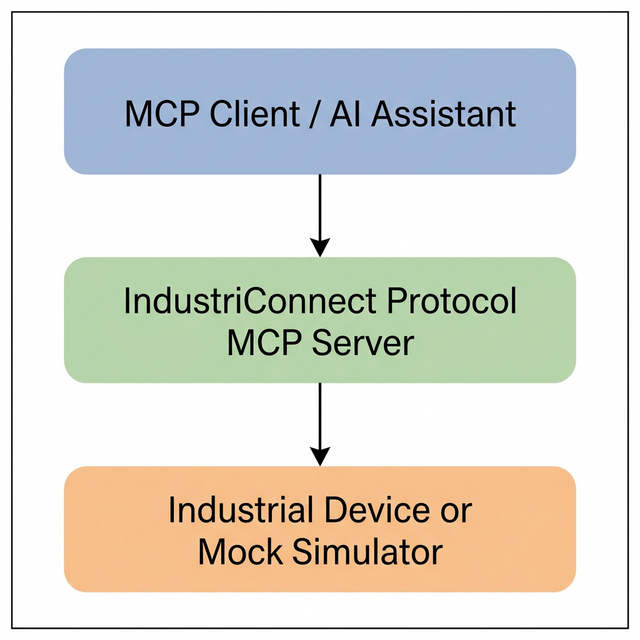
\includegraphics[width=0.88\linewidth]{figures/fig1_architecture.png}%
  }{%
    \figplaceholder{Three-Layer Architecture}{%
      Generate from: \texttt{figures/prompts/fig1\_architecture.md}}%
  }
  \caption{IndustriConnect three-layer architecture. The MCP client (AI
    assistant or web console) communicates with a protocol-specific MCP server
    over \texttt{stdio}; the server translates tool calls into native protocol
    operations directed at a real industrial device or its mock equivalent.}
  \label{fig:architecture}
\end{figure}

\textbf{Layer 1 — MCP Client.} The topmost layer consists of any MCP-compatible
client: Claude~Desktop, a custom LLM application, or the
\textit{mcp-manager-ui} web console described in Section~\ref{sec:ui}. The
client discovers available tools via \texttt{tools/list} and invokes them via
\texttt{tools/call}, receiving structured JSON responses without any knowledge
of the underlying industrial protocol.

\textbf{Layer 2 — Protocol MCP Server.} Each protocol is served by a dedicated
Python process implementing the MCP server interface via the FastMCP framework.
On receiving a \texttt{tools/call} request the server:
(i)~validates input parameters against the tool's JSON Schema;
(ii)~connects to the target device using the appropriate protocol library;
(iii)~executes the operation with timeout enforcement and retry logic;
(iv)~encodes the response in the unified envelope; and
(v)~returns the result over \texttt{stdio}.

\textbf{Layer 3 — Device or Mock.} The bottom layer is either a real industrial
device (PLC, RTU, sensor gateway) or one of the protocol-specific mock
simulators provided with the suite. The mock simulators implement the server
side of each protocol with realistic state and data, enabling complete stack
testing without physical hardware.

\subsection{FastMCP Framework}
\label{subsec:fastmcp}

All IndustriConnect MCP servers are implemented using FastMCP, a Python library
built on the MCP specification that provides:

\begin{itemize}
  \item \textbf{Declarative tool registration} via the \texttt{@mcp.tool()}
    decorator, with automatic JSON Schema generation from Python type hints.
  \item \textbf{Async-native execution} using Python's \texttt{asyncio},
    enabling non-blocking I/O for all protocol operations.
  \item \textbf{Lifespan management} through a context manager pattern that
    initialises protocol connections on server startup and releases them on
    shutdown.
  \item \textbf{Stdio transport} compatible with Claude~Desktop configuration
    and standard MCP runners.
\end{itemize}

Listing~\ref{lst:tool} illustrates the structure of a representative MCP tool
for typed Modbus register reads.

\begin{lstlisting}[style=pythonStyle, caption={Representative MCP tool definition for typed Modbus register read. FastMCP generates the JSON Schema for \texttt{tools/list} automatically from the type annotations.}, label={lst:tool}]
@mcp.tool()
async def read_holding_typed(
    address: int,
    dtype: str,          # int16 | uint16 | int32 | float32 | ...
    ctx: Context,
    count: int = 1,
    byteorder: str = "big",
    wordorder: str = "big",
    scale: float = 1.0,
    offset: float = 0.0,
    slave_id: int = DEFAULT_SLAVE_ID,
) -> Dict[str, Any]:
    """Read one or more typed values from Modbus holding registers."""
    t0 = time.monotonic()
    attempts = 0
    for attempt in range(MAX_RETRIES + 1):
        try:
            attempts += 1
            result = await _read_and_decode(
                address, count, dtype, byteorder, wordorder
            )
            return {
                "success": True,
                "data": {"values": result, "address": address},
                "error": None,
                "meta": {
                    "latency_ms": round((time.monotonic() - t0) * 1000, 2),
                    "attempts": attempts,
                },
            }
        except ModbusException as exc:
            if attempt == MAX_RETRIES:
                return _error_envelope(str(exc), t0, attempts)
            await asyncio.sleep(RETRY_BACKOFF_BASE ** attempt)
\end{lstlisting}

\subsection{Unified Response Envelope}
\label{subsec:envelope}

Every tool in every protocol module returns a JSON object with the same
four-field structure illustrated in Figure~\ref{fig:envelope} and
Listing~\ref{lst:envelope}.

\begin{figure}[h!]
  \centering
  \IfFileExists{figures/fig2_response_envelope.png}{%
    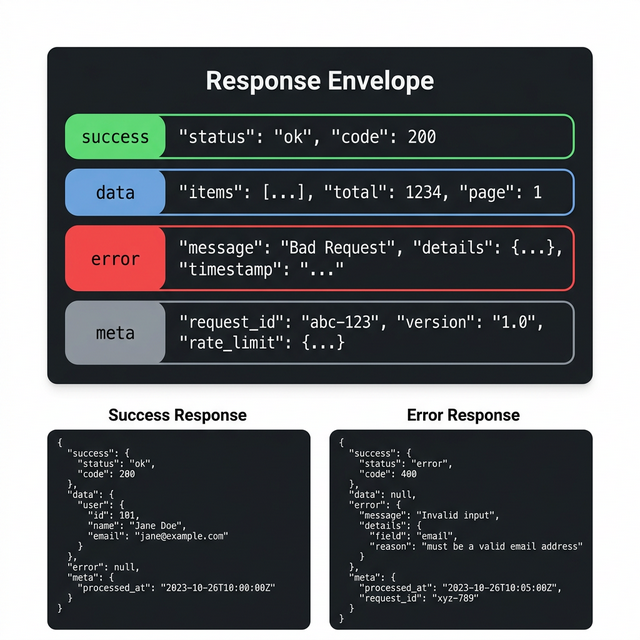
\includegraphics[width=0.82\linewidth]{figures/fig2_response_envelope.png}%
  }{%
    \figplaceholder{Response Envelope Visualisation}{%
      Generate from: \texttt{figures/prompts/fig2\_response\_envelope.md}}%
  }
  \caption{Unified response envelope returned by every IndustriConnect tool.
    The four fields provide success status, protocol-specific payload, error
    description, and operational metadata (latency, retry count).}
  \label{fig:envelope}
\end{figure}

\begin{lstlisting}[style=jsonStyle, caption={Unified response envelope — example for a Modbus holding register read.}, label={lst:envelope}]
{
  "success": true,
  "data": {
    "values": [3.14, 2.72],
    "address": 100,
    "dtype": "float32"
  },
  "error": null,
  "meta": {
    "latency_ms": 12.4,
    "attempts": 1,
    "raw": {}
  }
}
\end{lstlisting}

The \texttt{success} boolean allows the LLM to branch on failure without
parsing error strings. The \texttt{error} field carries a human-readable
exception message when \texttt{success} is \texttt{false}, enabling
conversational error reporting. The \texttt{meta} field exposes operational
telemetry—round-trip latency and retry count—that can be surfaced to
operators or logged for observability.

\subsection{Configuration Model}
\label{subsec:config}

Protocol servers are configured entirely through environment variables and
optional \texttt{.env} files. No protocol-specific configuration is compiled
into the server binary. For example, the Modbus server reads:

\begin{itemize}[noitemsep]
  \item \texttt{MODBUS\_TYPE} — connection type (\texttt{tcp}, \texttt{udp},
    \texttt{serial})
  \item \texttt{MODBUS\_HOST}, \texttt{MODBUS\_PORT} — network target
  \item \texttt{MODBUS\_DEFAULT\_SLAVE\_ID} — default device address
  \item \texttt{MODBUS\_MAX\_RETRIES}, \texttt{MODBUS\_TIMEOUT} — reliability
  \item \texttt{MODBUS\_WRITES\_ENABLED} — write-enable flag (safety gate)
  \item \texttt{REGISTER\_MAP\_FILE} — optional JSON tag map path
\end{itemize}

This separation allows the same server binary to target a mock device in
development, a staging copy, or a live PLC in production by changing only
environment variables—a property that substantially simplifies deployment
pipelines~\citep{humble2010continuous}.

Optional JSON \emph{tag maps} allow operators to define named aliases for
raw addresses:

\begin{lstlisting}[style=jsonStyle, caption={Example tag map entry for named Modbus register access.}, label={lst:tagmap}]
{
  "pump_speed_rpm": {
    "type": "holding",
    "address": 100,
    "dtype": "float32",
    "scale": 0.1,
    "description": "Pump shaft speed in RPM"
  }
}
\end{lstlisting}

Tag maps abstract raw addresses from AI-facing tool calls, enabling prompts
such as ``read the pump\_speed\_rpm'' rather than ``read float32 at holding
register 100''.

\subsection{Reliability Patterns}
\label{subsec:reliability}

Industrial field networks are subject to noise, transient faults, and
reconnection delays that are uncommon in IT environments. IndustriConnect
implements four reliability mechanisms shared across all protocol modules:

\textbf{Exponential-backoff retry.} Each tool retries on transient errors
up to \texttt{MAX\_RETRIES} times with a configurable backoff base (default
$b=2$\,s), waiting $b^{k}$ seconds after the $k$-th failure.

\textbf{Protocol-limit chunking.} Protocols such as Modbus impose maximum
payload sizes (125 registers per read, 2000 coils per read). Tools that
accept large ranges automatically split the request into legal-sized chunks,
reassemble the responses, and return a single result.

\textbf{Per-operation timeouts.} Every protocol call is wrapped with an
\texttt{asyncio.wait\_for} timeout fence, preventing indefinite blocking on
unresponsive devices.

\textbf{Automatic reconnection.} Client wrapper classes detect stale
connections and re-establish them transparently before retrying the failed
operation, so that short network interruptions are invisible to the AI client.

%% ─── 4. PROTOCOL IMPLEMENTATIONS ────────────────────────────────────────────
\section{Protocol Implementations}
\label{sec:protocols}

Table~\ref{tab:protocols} summarises the nine protocol modules.
Figure~\ref{fig:protocol_map} shows their relationships within the suite.
The following subsections describe each module's design decisions.

\begin{table*}[t!]
  \centering
  \caption{Protocol module summary. Tool count refers to the number of MCP
    tools exposed by each server; application domain indicates the primary
    industrial sector served.}
  \label{tab:protocols}
  \renewcommand{\arraystretch}{1.25}
  \resizebox{\textwidth}{!}{%
  \begin{tabular}{@{}lllrl@{}}
    \toprule
    \textbf{Protocol} & \textbf{Transport} & \textbf{Python Library} &
    \textbf{Tools} & \textbf{Application Domain} \\
    \midrule
    Modbus            & TCP / UDP / Serial  & \texttt{pymodbus}         & 14+ & Manufacturing, process, energy \\
    MQTT + Sparkplug~B& TCP (broker)        & \texttt{paho-mqtt}, \texttt{protobuf} & 10+ & IIoT telemetry, edge computing \\
    OPC~UA            & TCP (binary)        & \texttt{asyncua}          & 8   & Unified data access, I4.0 \\
    BACnet/IP         & UDP/IP              & \texttt{BAC0}             & 6   & Building automation \\
    DNP3              & TCP / Serial        & \texttt{pydnp3}           & 7   & Power utility SCADA \\
    EtherCAT          & Ethernet (raw)      & \texttt{PySOEM}           & 8   & Motion control, robotics \\
    EtherNet/IP       & TCP/IP              & \texttt{pycomm3}          & 7   & Rockwell/Allen-Bradley PLCs \\
    PROFIBUS DP/PA    & RS-485 / USB        & \texttt{pyserial}         & 6   & Process, discrete manufacturing \\
    PROFINET          & Ethernet            & \texttt{scapy}, \texttt{lxml} & 7 & Siemens factory automation \\
    Siemens S7comm    & ISO-on-TCP          & \texttt{python-snap7}     & 12  & Siemens S7 PLCs \\
    \bottomrule
  \end{tabular}}
\end{table*}

\begin{figure}[h!]
  \centering
  \IfFileExists{figures/fig3_protocol_map.png}{%
    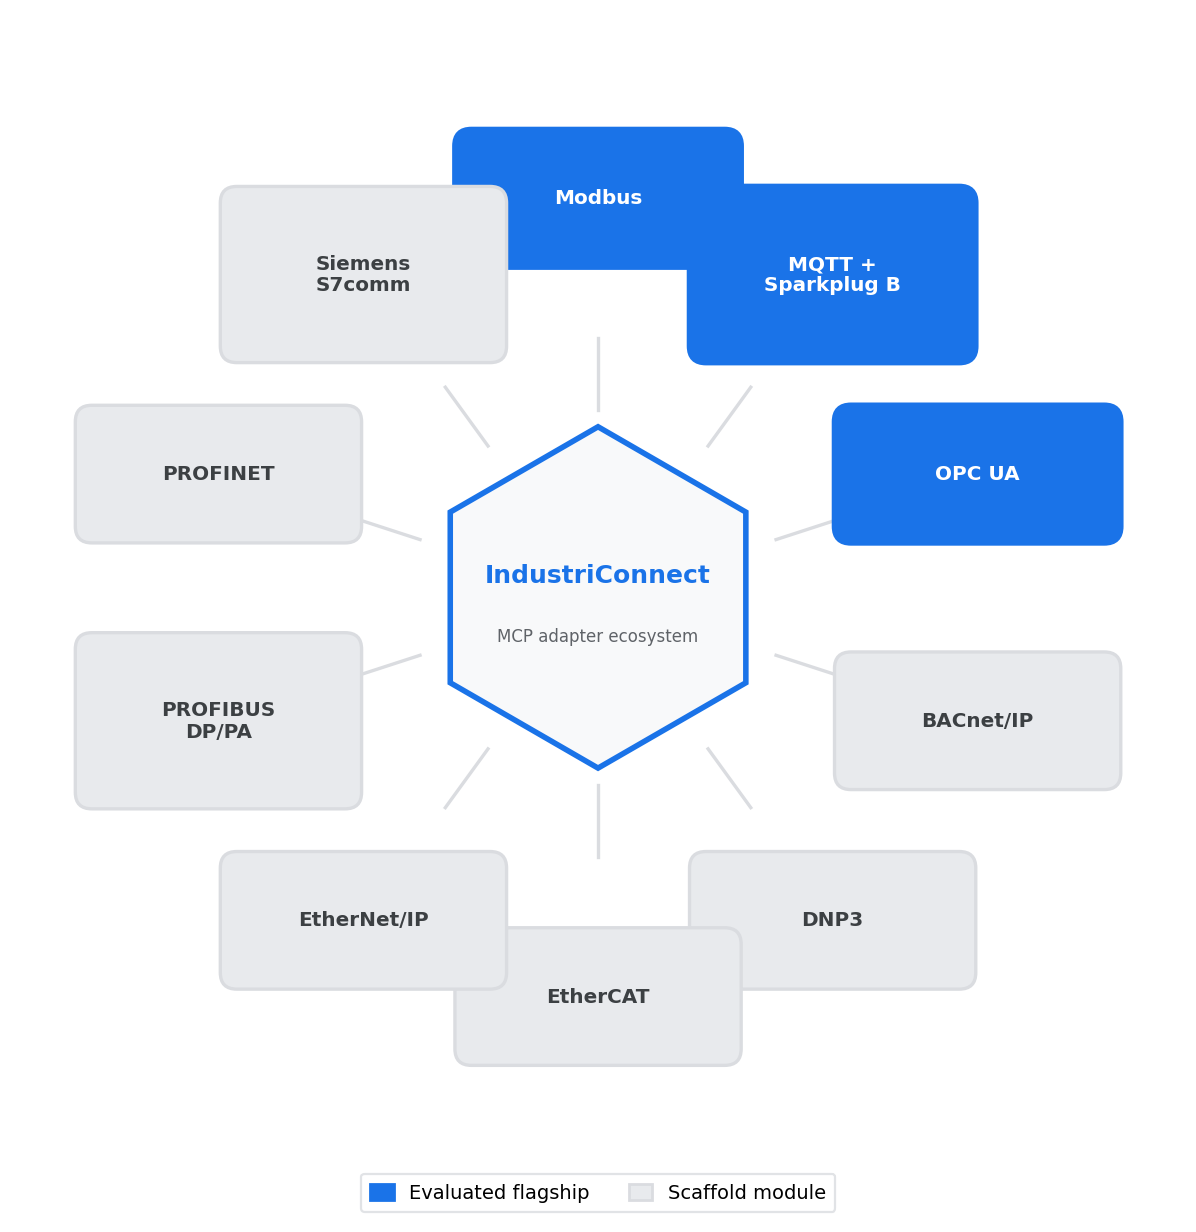
\includegraphics[width=0.90\linewidth]{figures/fig3_protocol_map.png}%
  }{%
    \figplaceholder{Protocol Ecosystem Map}{%
      Generate from: \texttt{figures/prompts/fig3\_protocol\_map.md}}%
  }
  \caption{IndustriConnect protocol ecosystem. Each spoke represents a
    dedicated MCP server module connecting the AI layer to a distinct
    industrial protocol domain.}
  \label{fig:protocol_map}
\end{figure}

\subsection{Modbus TCP/RTU/UDP}
\label{subsec:modbus}

Modbus is implemented using \texttt{pymodbus}~($\geq$3.9.2) with full support
for TCP, UDP, and serial RTU/ASCII transports, selectable via the
\texttt{MODBUS\_TYPE} environment variable. The server exposes tools covering
all four Modbus data objects: coils (function codes 1/5/15), discrete inputs
(FC~2), holding registers (FC~3/6/16), and input registers (FC~4). Advanced
typed read and write tools accept a \texttt{dtype} parameter
(\texttt{int16}, \texttt{uint16}, \texttt{int32}, \texttt{uint32},
\texttt{int64}, \texttt{uint64}, \texttt{float32}, \texttt{float64}) and apply
configurable byte-order and word-order transformations using
\texttt{BinaryPayloadDecoder}/\texttt{Builder} from \texttt{pymodbus}, along
with linear scale-and-offset correction. A \texttt{mask\_write\_register} tool
exposes the Modbus function-code~22 bitwise mask operation, enabling atomic
bit-field manipulation without read-modify-write races. Device identification
is exposed via the MEI~0x2B/0x0E function (FC~43). Tag maps provide symbolic
named access over the register address space, enabling prompts at the
\emph{process variable} level rather than the register level.

\subsection{MQTT + Sparkplug~B}
\label{subsec:mqtt}

The MQTT module wraps \texttt{paho-mqtt} with a connection manager that
handles broker authentication, TLS configuration, clean-session management,
and exponential-backoff reconnection. Standard tools cover
\texttt{publish\_message} (QoS~0--2, retain flag), \texttt{subscribe\_topic},
\texttt{unsubscribe\_topic}, \texttt{list\_subscriptions}, and
\texttt{get\_broker\_info}. The Sparkplug~B extension implements the full
Eclipse Tahu specification lifecycle: NBIRTH (node birth certificate),
DBIRTH (device birth certificate), NDATA (node data update), DDATA (device
data update), NCMD (node command), DCMD (device command), NDEATH, and DDEATH.
Sparkplug~B payloads are encoded and decoded using hand-crafted Protocol
Buffer serialisation, supporting metric types \texttt{int32}, \texttt{float},
\texttt{boolean}, and \texttt{string}. Sequence numbers are managed
automatically with 0--255 rollover. The design enables AI assistants to
participate as Sparkplug~B edge nodes, publishing structured telemetry and
responding to command metrics.

\subsection{OPC~UA}
\label{subsec:opcua}

The OPC~UA server wraps the \texttt{asyncua} library, providing fully
asynchronous node access. Tools include \texttt{read\_opcua\_node},
\texttt{write\_opcua\_node}, \texttt{browse\_opcua\_node\_children}, and
\texttt{call\_opcua\_method}, enabling AI agents to navigate the OPC~UA
address space, invoke remote methods on PLCs (e.g., motor start/stop
procedures), and read arbitrary node values by NodeId. Batch tools
\texttt{read\_multiple\_opcua\_nodes} and \texttt{write\_multiple\_opcua\_nodes}
accept arrays of NodeIds and execute grouped operations in a single tool call,
reducing round-trips for telemetry collection scenarios. A
\texttt{get\_all\_variables} tool performs full address-space discovery and
returns all variable nodes with their names, data types, and current values.
OPC~UA's native information model provides the data typing and hierarchy that
Modbus lacks, making it suitable for the highest-level AI reasoning tasks over
heterogeneous PLC data~\citep{cavalieri2013opcua}.

\subsection{BACnet/IP}
\label{subsec:bacnet}

The BACnet module uses the \texttt{BAC0} library to implement a BACnet/IP
client. \texttt{discover\_devices} broadcasts Who-Is requests across the
subnet and returns a list of device instance numbers with configurable timeout.
\texttt{read\_property} and \texttt{write\_property} access any object/property
combination using the standard quadruple (device\_id, object\_type,
object\_instance, property\_id), with write priority levels (1--16) supported
per the BACnet commandable property model. An optional JSON object map file
provides named aliases (e.g., ``zone\_3\_setpoint'') that resolve to
device/object/property triplets, simplifying AI prompts in building automation
scenarios. Change-of-value (COV) subscription and alarm monitoring are
identified as the primary directions for future development.

\subsection{DNP3}
\label{subsec:dnp3}

The DNP3 module operates as a DNP3 master station using \texttt{pydnp3} over
both TCP and serial transports. It exposes read tools for all three standard
data object groups: binary inputs (Group~1), analog inputs (Group~30), and
counters (Group~20). Control output operations (Group~12 CROB — Control Relay
Output Block, and Group~41 Analog Outputs) enable AI-driven setpoint and
switch control in power utility SCADA environments. Point maps provide
named access analogous to Modbus tag maps. The master/outstation addresses,
link-layer timeouts, and retry policy are configurable, and the mock outstation
provides a safe sandbox for SCADA workflow development without access to
substation equipment.

\subsection{EtherCAT}
\label{subsec:ethercat}

EtherCAT access is implemented via \texttt{PySOEM}, a Python binding for the
SOEM (Simple Open EtherCAT Master) library. Network scanning discovers
connected slaves and reports their vendor ID, product code, revision, and
assigned position. Per-slave process data objects (PDOs) support cyclic
read/write of mapped I/O variables. Service data objects (SDOs) provide
acyclic parameter access by index and subindex for configuration and
diagnostics. ESI (Electronic Slave Information) file parsing exposes
human-readable parameter descriptions. A configurable cycle time controls
the PDO exchange period. Due to raw Ethernet socket requirements, EtherCAT
operations require elevated network privileges (\texttt{CAP\_NET\_RAW} on
Linux) or administrator rights, a constraint documented clearly in the
tool descriptions.

\subsection{EtherNet/IP}
\label{subsec:ethernetip}

EtherNet/IP (Common Industrial Protocol) access targets Rockwell/Allen-Bradley
controllers using the \texttt{pycomm3} library. The primary tools
\texttt{read\_tag} and \texttt{write\_tag} accept symbolic tag names as used in
Logix~5000 ladder logic programs, supporting scalar, array, and structured
(User Defined Type, UDT) tags. Array slices can be read by specifying element
count and offset. Tag discovery stubs enumerate the controller's tag database
for exploration. The design follows the ``controller tag'' abstraction familiar
to Rockwell engineers, hiding the underlying CIP (Common Industrial Protocol)
messaging from the AI layer.

\subsection{PROFIBUS DP/PA}
\label{subsec:profibus}

PROFIBUS is accessed via USB-to-RS-485 or native PROFIBUS adapters using
\texttt{pyserial} as the physical transport. The server supports Generic
Station Description (GSD) file parsing to resolve slave device capabilities
and module configurations. Bus scanning identifies active slave addresses and
their diagnostic information. Cyclic I/O data exchange reads input process
data and writes output process data for mapped slaves. A
\texttt{PROFIBUS\_MOCK=true} environment variable activates a software mock
mode for development environments without physical bus adapters, reflecting
the suite-wide mock-first philosophy.

\subsection{PROFINET}
\label{subsec:profinet}

PROFINET device discovery uses the DCP (Discovery and Configuration Protocol)
implemented with the \texttt{scapy} packet manipulation library, enabling
broadcast identification of PROFINET IO devices on the local Ethernet segment.
GSDML (PROFINET station description) files are parsed using \texttt{lxml}
to extract device metadata, slot/subslot module configurations, and parameter
descriptions. Module management tools configure the IO device's application
relation, and cyclic I/O communication exchanges process data with configured
submodules. PROFINET similarly requires raw Ethernet socket privileges for
DCP frame construction.

\subsection{Siemens S7comm}
\label{subsec:s7comm}

S7comm access is provided via \texttt{python-snap7}, a Python binding for the
libsnap7 library, targeting S7-300, S7-400, S7-1200, and S7-1500 PLCs.
Data block (DB) access tools \texttt{read\_db} and \texttt{write\_db} transfer
raw byte arrays by DB number, offset, and size. \texttt{read\_db\_typed}
accepts a \texttt{dtype} parameter (\texttt{BOOL}, \texttt{BYTE},
\texttt{CHAR}, \texttt{WORD}, \texttt{INT}, \texttt{DINT}, \texttt{REAL},
\texttt{STRING}) and applies S7-specific binary parsing including bit addressing
within bytes. Separate tools access process input/output areas, the marker
(M) memory area, and timer/counter special function areas. \texttt{read\_szl}
reads System Zone List records for diagnostics (CPU model, module state, fault
history). Tag maps support named DB access patterns. Write operations and
system-level commands are individually guarded by environment flags
(\texttt{S7\_WRITES\_ENABLED}, \texttt{S7\_SYSTEM\_CMDS\_ENABLED}) for
operational safety.

%% ─── 5. MOCK-FIRST DEVELOPMENT ───────────────────────────────────────────────
\section{Mock-First Development Methodology}
\label{sec:mock}

\begin{figure}[h!]
  \centering
  \IfFileExists{figures/fig4_mock_lifecycle.png}{%
    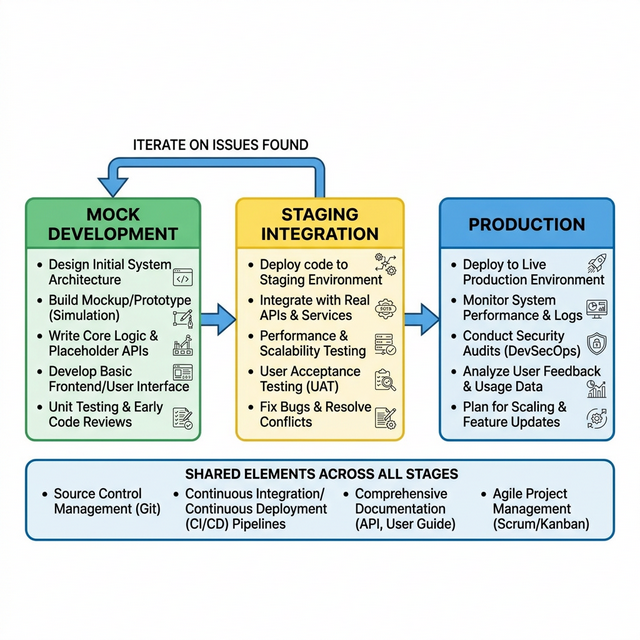
\includegraphics[width=0.88\linewidth]{figures/fig4_mock_lifecycle.png}%
  }{%
    \figplaceholder{Mock-First Development Lifecycle}{%
      Generate from: \texttt{figures/prompts/fig4\_mock\_lifecycle.md}}%
  }
  \caption{Mock-first development lifecycle. Prompts and workflows are
    developed and validated against mock simulators before being progressively
    promoted to staging and production environments.}
  \label{fig:mock-lifecycle}
\end{figure}

\subsection{Rationale}
\label{subsec:mock-rationale}

Industrial OT systems present a fundamental challenge for AI workflow
development: access to production equipment is restricted for safety, cost,
and availability reasons; staging environments are scarce; and physical devices
cannot be rolled back after a mis-directed write. The mock-first methodology
addresses this by mandating that every protocol module ships with a
software-only device simulator that faithfully replicates the server side of
the protocol~\citep{digital_twin_benefits}.

The consequence for AI development is significant: prompt engineers, data
scientists, and system integrators can develop, iterate, and validate complete
end-to-end workflows on a laptop without access to any physical hardware.
Failures are deterministic, recoverable, and incur no physical risk.

\subsection{Mock Device Design}
\label{subsec:mock-design}

Each mock device is designed according to four principles:

\textbf{Protocol fidelity.} The mock implements the full server-side state
machine of the protocol. The Modbus mock server is a fully compliant TCP slave
with realistic register state (pump speed, tank level, temperature, status
word). The OPC UA mock server builds a rich information model hierarchy with
sensor, actuator, and alarm nodes. The MQTT mock deploys a complete broker
plus Sparkplug~B edge node simulation with periodic data updates.

\textbf{Process realism.} Mock registers are not random; they reflect plausible
process behaviour. The Modbus mock simulates pump/tank dynamics. The S7comm
mock contains data blocks structured as a real PLC program would define them.
This trains AI prompts on realistic value ranges and update patterns.

\textbf{Standalone operation.} Each mock can be started with a single
\texttt{uv run <entrypoint>} command, with no dependency on the MCP server or
any AI client. This enables unit-level testing of the mock in isolation.

\textbf{Deterministic reproducibility.} Mock state is initialised from fixed
defaults and evolves predictably, enabling regression tests that compare AI
tool responses across versions.

\subsection{Development and Deployment Lifecycle}
\label{subsec:mock-lifecycle}

The recommended three-stage lifecycle, illustrated in
Figure~\ref{fig:mock-lifecycle}, is:

\begin{enumerate}
  \item \textbf{Mock stage}: The MCP server targets the mock device. AI
    prompts are developed, refined, and validated. Errors are debugged
    without hardware risk.
  \item \textbf{Staging stage}: The MCP server is reconfigured (by changing
    environment variables) to target a staging or shadow copy of the
    production system. Integration-level testing validates that the prompt
    strategies developed against the mock also work against real protocol
    behaviour.
  \item \textbf{Production stage}: The final configuration targets live
    field devices. Write-enable and system-command flags are explicitly
    reviewed and set. Monitoring on latency, error rate, and call frequency
    is established.
\end{enumerate}

%% ─── 6. MCP MANAGER UI ───────────────────────────────────────────────────────
\section{MCP Manager User Interface}
\label{sec:ui}

\begin{figure}[h!]
  \centering
  \IfFileExists{figures/fig5_mcp_manager_ui.png}{%
    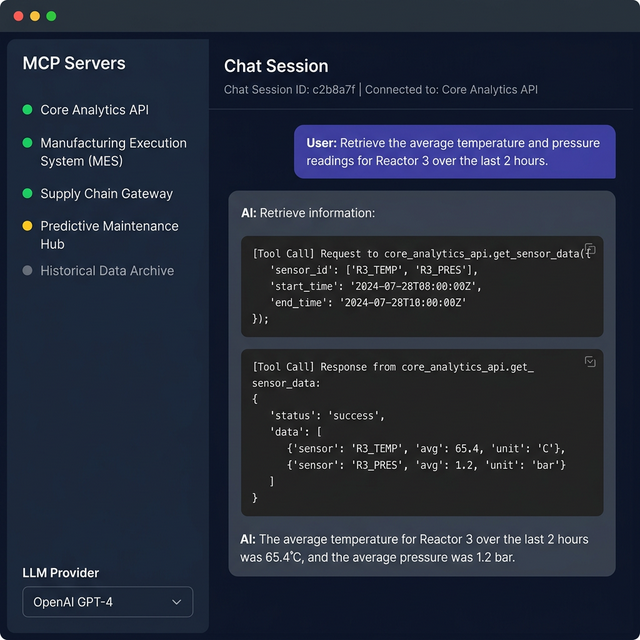
\includegraphics[width=0.90\linewidth]{figures/fig5_mcp_manager_ui.png}%
  }{%
    \figplaceholder{mcp-manager-ui Screenshot}{%
      Generate from: \texttt{figures/prompts/fig5\_mcp\_manager\_ui.md}}%
  }
  \caption{The \textit{mcp-manager-ui} web console. The left sidebar lists
    configured MCP servers with live connection status indicators; the main
    panel provides a chat interface connected to the selected LLM; tool call
    results are displayed as structured cards.}
  \label{fig:ui}
\end{figure}

The \textit{mcp-manager-ui} is a browser-based management console that
provides a unified interface for working with IndustriConnect protocol servers
and other MCP backends. It is implemented as a React + TypeScript single-page
application built with Vite, communicating with a lightweight Node.js backend
via HTTP REST and WebSocket.

\textbf{Server management.} The sidebar lists configured MCP servers with
real-time connection status indicators. Servers are added via a manual
configuration form, by importing a Cursor-style JSON config block, or through
a JSON editor for advanced users. Each server entry shows its configured
protocol, connection state, and tool count.

\textbf{LLM chat integration.} The main panel provides a session-based chat
interface. Users select from cloud LLM providers (Anthropic Claude, OpenAI
GPT, Google Gemini) or a locally running Ollama instance. API keys are stored
in browser local storage or loaded from environment variables. Messages,
tool call arguments, and tool responses are displayed inline, giving operators
a transparent view of the AI's reasoning and device interactions.

\textbf{Tool schema inspection.} A dedicated tool inspector view renders the
JSON Schema for each available tool, enabling operators to understand
parameter types and constraints before issuing commands.

The backend Node.js process acts as a secure proxy between the browser and
local MCP servers, preventing direct browser access to local process stdio.
WebSocket connections provide real-time streaming of LLM tokens and tool
results.

%% ─── 7. USE CASES ────────────────────────────────────────────────────────────
\section{Use Cases and Evaluation}
\label{sec:usecases}

This section presents four representative use cases that illustrate the
capability of IndustriConnect for AI-assisted industrial operations.

\subsection{Predictive Maintenance via Cross-Protocol Data Collection}
\label{subsec:uc-predictive}

An AI assistant is connected simultaneously to a Modbus MCP server (targeting
a variable-frequency drive) and an OPC~UA MCP server (targeting the plant's
historian). The operator prompts: ``Compare the current drive current draw
with the historical baseline for this time of day and report any anomaly.''
The assistant (i)~calls \texttt{read\_holding\_typed} on the Modbus server to
fetch instantaneous motor current, (ii)~calls \texttt{read\_multiple\_opcua\_nodes}
on the OPC~UA server to retrieve historical statistics, (iii)~computes the
deviation, and (iv)~returns a natural language summary flagging a 15\% above-baseline
reading as a potential bearing wear indicator.

This scenario demonstrates the composability of cross-protocol tool chains and
the value of the unified response envelope: the LLM receives identically
structured JSON from both protocols, enabling straightforward numeric
comparison without protocol-specific parsing logic.

\subsection{IIoT Telemetry Monitoring with MQTT/Sparkplug~B}
\label{subsec:uc-mqtt}

A manufacturing plant publishes machine state via Sparkplug~B edge nodes. The
AI assistant subscribes to relevant topics using \texttt{subscribe\_topic},
receives DDATA payloads via the MQTT MCP server, and decodes the Protobuf
metrics to extract throughput, reject rate, and downtime events. The assistant
then generates a shift summary report in natural language, identifies which
lines underperformed against targets, and proposes corrective actions. The
full Sparkplug~B lifecycle support means the assistant can also send NCMD
messages to trigger remote procedure calls on the edge nodes.

\subsection{Cross-Protocol Data Reconciliation}
\label{subsec:uc-reconcile}

A commissioning engineer suspects that an OPC~UA server's cached value for a
temperature setpoint differs from the value actually stored in the PLC data
block. Using IndustriConnect, the assistant reads the same physical variable
via both the OPC~UA server (\texttt{read\_opcua\_node}) and directly from the
S7comm PLC (\texttt{read\_db\_typed}), compares the results, and reports any
discrepancy. This ``dual read'' pattern, which would require significant
custom integration code in a traditional system, is expressed as a natural
language question and resolved in a single assistant turn.

\subsection{AI-Assisted Fault Diagnosis}
\label{subsec:uc-diagnosis}

An operator reports an intermittent fault on a Siemens PLC line. The AI
assistant uses \texttt{read\_szl} to fetch the PLC's fault buffer (SZL~ID
0x00A0), parses the diagnostic records, and identifies a recurring I/O module
communication timeout in rack~2, slot~4. It then calls
\texttt{read\_input} for the affected I/O area to confirm the current read
failure, and recommends a specific module reseating procedure based on
the fault code. This workflow replaces a multi-step manual process requiring
direct PLC access with a conversational, tool-driven diagnostic session.

\subsection{Discussion}
\label{subsec:discussion}

These use cases share a common pattern: the AI assistant decomposes a
high-level operator intent into a sequence of structured tool calls, assembles
the results, and presents actionable insight in natural language. The latency
of IndustriConnect tool calls is dominated by network round-trip time to the
field device; in local-network conditions, typical tool call latency ranges from
5\,ms (Modbus TCP single register read) to 200\,ms (OPC~UA full address-space
discovery), well within human conversational timescales.

Write operations are guarded by environment flags (\texttt{WRITES\_ENABLED})
that must be explicitly set for each deployment; this prevents accidental
modification of process state during diagnostic sessions. Future work on
operation approval flows and audit logging would further strengthen the safety
model for production use.

%% ─── 8. RELATED WORK ─────────────────────────────────────────────────────────
\section{Related Work}
\label{sec:related}

\textbf{Industrial protocol libraries.} The Python ecosystem provides mature
client libraries for individual protocols: \texttt{pymodbus} for Modbus,
\texttt{asyncua} for OPC~UA, \texttt{python-snap7} for S7comm, and
\texttt{pycomm3} for EtherNet/IP. IndustriConnect adds the MCP layer above
these libraries, exposing them as structured AI tools with a unified interface
and consistent reliability patterns.

\textbf{Industrial middleware and historians.} Commercial platforms such as
Inductive Automation Ignition, Node-RED, OSIsoft PI, and Kepware KEPServerEX
provide protocol normalisation and data historian functions~\citep{boyes2018iiot}.
These systems aggregate data from heterogeneous protocols into a unified
store or tag namespace. IndustriConnect is complementary: where historians
provide historical data storage and HMI visualisation, IndustriConnect focuses
specifically on AI-native, real-time tool-call access. IndustriConnect could
be configured to sit alongside a historian, with some tools reading live device
data and others querying the historian's OPC~UA or REST interface.

\textbf{IT/OT integration in Industry~4.0.} The integration of industrial
automation systems with IT infrastructure has been extensively studied in the
context of Industry~4.0~\citep{xu2018industry4, colombo2017cyberphysical}.
OPC~UA has emerged as the preferred normalisation layer~\citep{wollschlaeger2017future},
and digital twin frameworks increasingly rely on OPC~UA or MQTT as their
live-data backbone~\citep{fuller2020digital, tao2019digital}. IndustriConnect
treats OPC~UA as one of several equally supported protocols rather than an
exclusive normalisation point, preserving direct access to legacy fieldbuses
that may not have an OPC~UA gateway.

\textbf{LLM agents and tool use.} The capability of LLMs to invoke external
tools and APIs has been established across many application
domains~\citep{wuest2016ml}. Function-calling interfaces provided by OpenAI,
Anthropic, and Google enable structured tool invocation, but they are
provider-specific and not designed for the low-latency, schema-driven
interoperability that MCP provides. ReAct-style
agent loops~\citep{yao2022react} and tool-augmented language
models~\citep{schick2023toolformer} demonstrate the reasoning patterns that
IndustriConnect is designed to support; the suite provides the protocol-level
infrastructure that those patterns require in industrial settings.

\textbf{Digital twins and simulation.} Digital twin research advocates
maintaining a live synchronised replica of physical assets for
monitoring, prediction, and control~\citep{fuller2020digital, tao2019digital,
pivoto2021cps}. IndustriConnect's mock devices are lightweight process
simulators rather than full digital twins, but they serve a complementary
function: enabling AI workflow development without physical access, with the
possibility of upgrading to a full digital twin back-end in production.

\textbf{Industrial cybersecurity.} Connecting AI systems to OT networks
introduces cybersecurity considerations documented in the industrial security
literature~\citep{ralston2007scada}. IndustriConnect's write-enable flags
and mock-first development philosophy partially address operational safety;
full security hardening (network segmentation, TLS, authentication, audit
logging) is identified as future work.

%% ─── 9. CONCLUSION ───────────────────────────────────────────────────────────
\section{Conclusion and Future Work}
\label{sec:conclusion}

This paper has presented \textbf{IndustriConnect}, a suite of Model Context
Protocol servers that enables AI assistants to communicate with the full
breadth of industrial automation protocols through a unified, structured tool
interface. The five principal contributions—nine protocol MCP servers, a
unified response envelope, a mock-first development methodology, industrial
reliability patterns, and a web management console—collectively address the
protocol gap that has prevented AI assistants from participating meaningfully
in operational technology environments.

The suite demonstrates that MCP's schema-driven, transport-agnostic architecture
is well suited to industrial integration: tool schemas give AI agents the
structural context to invoke protocol operations correctly; the unified response
envelope enables cross-protocol reasoning without protocol-specific parsing; and
the mock devices enable complete end-to-end AI workflow development without
hardware access or production risk.

\textbf{Future work} falls into four categories:

\begin{enumerate}
  \item \textbf{Security hardening}: TLS support for protocol connections where
    available (OPC~UA, MQTT), stronger authentication, fine-grained write
    permission models, and operation approval flows with audit logging.
  \item \textbf{Expanded tool coverage}: Additional Modbus function codes,
    extended S7comm SZL area support, DNP3 file transfer and time
    synchronisation, and BACnet COV subscription and alarm management.
  \item \textbf{Richer mock scenarios}: Fault injection (connection drops,
    CRC errors, slave exception responses), alarm simulation, degraded-mode
    operation, and multi-device topologies for realistic end-to-end testing.
  \item \textbf{Empirical evaluation}: Structured experiments measuring
    AI task completion rate, tool call accuracy, and latency across the
    protocol suite on representative hardware, including comparison with
    human-operator baselines for diagnostic tasks.
\end{enumerate}

IndustriConnect is released as open source and is available at
\url{https://github.com/NordicAgents/IndustriConnect}. Contributions in the form of
additional tool coverage, improved mock scenarios, and protocol extensions are
welcomed.

%% ─── Acknowledgements ────────────────────────────────────────────────────────
\section*{Acknowledgements}
The authors thank the maintainers of the open-source protocol libraries on
which IndustriConnect depends: \texttt{pymodbus}, \texttt{asyncua},
\texttt{python-snap7}, \texttt{pycomm3}, \texttt{pydnp3}, \texttt{PySOEM},
\texttt{BAC0}, \texttt{paho-mqtt}, and \texttt{scapy}.

%% ─── References ──────────────────────────────────────────────────────────────
\bibliographystyle{plainnat}
\bibliography{references}

\end{document}
